\chapter{Giới thiệu}
Chương này trình bày tổng quan về bài toán hỗ trợ chẩn đoán bệnh lý trên ảnh X-quang bằng học sâu đa phương thức, đặc biệt trong bối cảnh dữ liệu y tế thường có tính phức tạp cao và phụ thuộc mạnh vào kinh nghiệm của bác sĩ trong quá trình phân tích. Bên cạnh thông tin hình ảnh, quá trình chẩn đoán thực tế còn yêu cầu kết hợp thêm các thông tin lâm sàng và báo cáo y khoa nhằm đưa ra đánh giá toàn diện về tình trạng bệnh nhân. Tuy nhiên, việc khai thác đồng thời nhiều nguồn dữ liệu khác nhau vẫn còn là một thách thức lớn đối với các hệ thống học sâu hiện nay.

Xuất phát từ thực tế đó, khóa luận hướng đến nghiên cứu và xây dựng một hệ thống học sâu đa phương thức kết hợp dữ liệu hình ảnh X-quang và thông tin văn bản lâm sàng nhằm nâng cao hiệu năng phân loại và hỗ trợ chẩn đoán. Đồng thời, đề tài cũng khảo sát các phương pháp tinh chỉnh mô hình tiền huấn luyện, cơ chế dung hợp dữ liệu và cơ chế giải thích nhằm tăng khả năng tận dụng tri thức nền cũng như cải thiện tính minh bạch trong quá trình suy luận của mô hình. Kết quả nghiên cứu được kỳ vọng góp phần xây dựng một hệ thống hỗ trợ chẩn đoán có độ chính xác cao, khả năng giải thích tốt và tạo tiền đề cho việc ứng dụng các mô hình trí tuệ nhân tạo đa phương thức trong lĩnh vực y tế tại Việt Nam.
\label{Chapter1}

% Hệ xương đóng vai trò rất lớn trong việc nâng đỡ cơ thể, bảo vệ các cơ quan trọng yếu và đảm bảo khả năng vận động của con người. Do đó, chấn thương xương khớp và các bệnh lý về xương là một trong những vấn đề y tế phổ biến, đòi hỏi việc chẩn đoán phải được thực hiện nhanh chóng và chính xác. Trong thực hành lâm sàng, ảnh X-quang xương là phương tiện chẩn đoán hình ảnh cơ bản, phổ biến và có chi phí thấp, cho phép bác sĩ quan sát cấu trúc xương, phát hiện tổn thương và định hướng điều trị ngay từ giai đoạn đầu. Tuy nhiên, việc đọc và phân tích ảnh X-quang truyền thống hiện nay phụ thuộc rất lớn vào kinh nghiệm thực tiễn và sự tập trung của bác sĩ. Điều này dễ dẫn đến những sai sót không đáng có khi lượng bệnh nhân quá lớn gãy quá tải cho các y bác sĩ. 

% Để giải quyết các thách thức này, các nghiên cứu hiện nay đã ứng dụng các mô hình học sâu vào để giải quyết vấn đề đọc ảnh và đưa ra quyết định dựa trên thông tin trên ảnh. Tuy nhiên, các mô hình này vẫn chưa đạt được hiệu quả đủ để đưa vào ứng dụng thực tế. Một trong các lý do chính đó là các mô hình chỉ mới tiếp cận được các thông tin trong ảnh, các y bác sĩ không chỉ dựa vào thông tin thông qua việc đọc ảnh mà còn dựa vào các thông tin từ nhiều nguồn bao gồm: thông tin từ bệnh nhân thông qua lời khai và khám lâm sàng sau đó các xét nghiệm cận lâm sàng như X-quang kèm với thông tin từ bác sĩ đọc ảnh để bổ trợ, từ đó giúp bác sĩ đưa ra chẩn đoán sơ khởi hay chẩn đoán chính xác. Dựa vào thực tế đó, các nghiên cứu hiện nay đang dần chuyển dịch sang hướng tiếp cận đa phương thức nhằm mô phỏng lại quá trình chẩn đoán của bác sĩ nhằm nâng cao hiệu năng của hệ thống.

% Khác với các mô hình đơn phương thức chỉ xử lý trên một phương thức như ảnh hay văn bản duy nhất, các mô hình đa phương thức có thể sử dụng nhiều phương thức và tìm ra sự tương quan giữa các phương thức nhằm tạo nên biểu diễn có ý nghĩa hơn từ đó nâng cao hiệu năng của hệ thống. Với thực tế lâm sàng hiện nay, các mô hình nghiên cứu tập trung vào kết hợp ngôn ngữ và hình ảnh hay còn được gọi là mô hình ngôn ngữ trực quan đang là các mô hình đang nhận được nhiều sự chú ý. 

% \section{Định nghĩa các khái niệm}
% \subsection{Thông tin lâm sàng}
% Thông tin lâm sàng là những dữ liệu thu thập trực tiếp qua quá trình bác sĩ thăm khám người bệnh, bao gồm việc khai thác bệnh sử và khám thực thể (nhìn, sờ, gõ, nghe) \cite{Dorland2011}. Dữ liệu này mang tính chất định hướng ban đầu, giúp bác sĩ khoanh vùng tổn thương và đưa ra các quyết định chỉ định thăm khám chuyên sâu tiếp theo \cite{Bickley2020_Bates}.
% \subsection{Thông tin cận lâm sàng}
% Thông tin cận lâm sàng là các dữ liệu khách quan thu được từ việc áp dụng các trang thiết bị và kỹ thuật y khoa hiện đại (như hình ảnh X-quang, cắt lớp, hay xét nghiệm sinh hóa) \cite{Dorland2011}. Nếu lâm sàng dùng để định hướng, thì cận lâm sàng cung cấp bằng chứng xác thực từ bên trong cơ thể để chẩn đoán chính xác bệnh lý.

% \section{Phát biểu bài toán}
% \subsection{Đầu vào (Input)}
% Hệ thống nhận vào các nguồn dữ liệu sau:
% \begin{itemize}
%     \item Thông tin lâm sàng bao gồm báo cáo cận lâm sàng, khám xét toàn thân, lý do vào viện của bệnh nhân.
%     \item Ảnh X-quang xương của bệnh nhân tương ứng.
%     \item Tập nhãn được định nghĩa trước.
% \end{itemize}
% \subsection{Đầu ra (Output)}
% Hệ thống sẽ sinh ra các nhãn sau:
% \begin{itemize}
%     \item Tỉ lệ mà ảnh và thông tin lâm sàng tương ứng thuộc vào các lớp được định nghĩa trước.
%     \item Ảnh trực quan hóa giải thích cho kết quả.
% \end{itemize}
% \subsection{Kiến trúc tổng quan}
% Với bài toán này, kiến trúc tổng quan của một mô hình học sâu đa phương thức được sử dụng bao gồm bốn thành phần chính: bộ mã hóa ảnh, bộ mã hóa văn bản, bộ dung hợp dữ liệu và bộ phân loại như được thể hiện ở Hình \ref{fig:pipeline}.

% \begin{figure}[H]
%     \centering
%     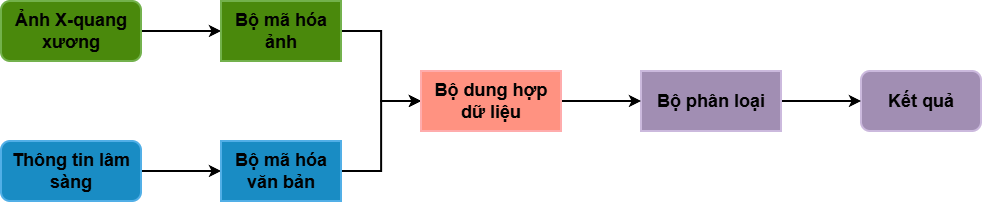
\includegraphics[width=1\linewidth]{images/Pipeline.png}
%     \caption{Khung chương trình tổng quát cho một hệ thống phân loại ảnh sử dụng học sâu đa phương thức}
%     \label{fig:pipeline}
% \end{figure}

% Trong đó, bộ mã hóa ảnh có chức năng rút trích đặc trưng từ ảnh đầu vào, bộ mã hóa văn bản có chức năng rút trích đặc trưng từ văn bản đầu vào, bộ dung hợp dữ liệu có chức năng dung hợp hay căn chỉnh các đặc trưng được rút trích từ hai phương thức dữ liệu trên để tạo ra một biểu diễn có ý nghĩa và có đầy đủ tính chất của phương thức đầu vào, đây cũng là mô-đun quan trọng nhất đối với một mô hình học sâu đa phương thức, cuối cùng là bộ phân loại, nhận biểu diễn đặc trưng chung của các phương thức đầu vào để phân loại và đưa ra kết quả cuối cùng.

% \section{Mục tiêu đề tài}

% Trong bối cảnh già hóa dân số và các tác nhân gây bệnh từ ô nhiễm và lối sống thiếu lành mạnh trong đời sống hiện đại, các bệnh lý về xương và chấn thương có thể ảnh hưởng trực tiếp đến đời sống và tính mạng dẫn đến việc chẩn đoán và tiên lượng để đưa ra hướng điều trị phù hợp đang trở thành gánh nặng cho các y bác sĩ, các hệ thống học sau đa phương thức tuy đã phát triển nhưng lại thiếu khả năng giải thích. Đề tài hướng đến phát triển một hệ thống phân loại ảnh X-quang có khả năng:
% \begin{itemize}
%     \item Đạt được độ chính xác cao trên các bộ dữ liệu nội bộ và quốc tế.
%     \item Có khả năng giải thích được kết quả.
%     \item Tích hợp kết quả để trợ giúp y bác sĩ trong quá trình chẩn đoán.
% \end{itemize}

% \section{Phạm vi của đề tài}

% Nội dung nghiên cứu của đề tài tập trung vào việc khảo sát các mô hình nền tảng và thiết kế, huấn luyện, tinh chỉnh, đánh giá kiến trúc được đề xuất trên ảnh X-quang xương và các bộ dữ liệu quốc tế để so sánh, đánh giá với các kiến trúc trước.

% Đối tượng nghiên cứu xoay quanh các thành phần bên trong một mạng học sâu đa phương thức bao gồm: bộ mã hóa ảnh, bộ mã hóa văn bản, bộ dung hợp dữ liệu và bộ phân loại, tập trung vào các phương pháp dung hợp dữ liệu hình ảnh và văn bản cùng với các phương pháp tinh chỉnh tham số cho các bộ mã hóa đã được huấn luyện trước nhằm tận dụng lại các tri thức đã có và nâng cao hiệu năng trên các tác vụ đích.

% Đề tài chủ yếu sử dụng các bộ dữ liệu cặp ảnh - văn bản, không có trường hợp thiếu đã được công bố và bộ dữ liệu nội bộ được thu thập và cung cấp bởi giảng viên có hợp tác với bệnh viện ở khu vực Thành phố Hồ Chí Minh, một số thông tin cơ bản về các bộ dữ liệu được thể hiện ở Bảng \ref{tab:datasets}. Nhóm sử dụng các bộ dữ liệu này nhằm đánh giá hiệu năng của kiến trúc đề xuất thông qua các độ đo phổ biến và tiến hành so sánh với các phương pháp trước đó nhằm chứng minh sự hiệu quả của phương pháp đề xuất.

% \begin{table}[htpb]
% \centering
% \resizebox{\textwidth}{!}{
% \begin{tabular}{|l|l|l|l|l|}
% \hline
% \multicolumn{1}{|c|}{\textbf{Bộ dữ liệu}} &
%   \textbf{Nguồn} &
%   \multicolumn{1}{c|}{\textbf{Loại dữ liệu}} &
%   \multicolumn{1}{c|}{\textbf{Số lượng mẫu}} &
%   \multicolumn{1}{c|}{\textbf{Số lượng lớp}} \\ \hline
% \begin{tabular}[c]{@{}l@{}}RSNA Pneumonia\\ (2018)\end{tabular} &
%   \begin{tabular}[c]{@{}l@{}}Radiological  Society \\ of North America\end{tabular} &
%   \begin{tabular}[c]{@{}l@{}}Ảnh X-quang ngực\\ metadata/tags\end{tabular} &
%   30,000 &
%   3 \\ \hline
% \begin{tabular}[c]{@{}l@{}}CheXpert\\ (2019)\end{tabular} &
%   \begin{tabular}[c]{@{}l@{}}Standford ML Group -\\ Stanford Hospital\end{tabular} &
%   \begin{tabular}[c]{@{}l@{}}Ảnh X-quang ngực\\ Báo cáo đọc ảnh\end{tabular} &
%   224,316 &
%   14 \\ \hline
% \begin{tabular}[c]{@{}l@{}}MIMIC-CXR v2\\ (2019)\end{tabular} &
%   \begin{tabular}[c]{@{}l@{}}Beth Israel Deaconess \\ Medical Center\end{tabular} &
%   \begin{tabular}[c]{@{}l@{}}Ảnh X-quang ngực\\ Báo cáo đọc ảnh\end{tabular} &
%   227,835 &
%   14 \\ \hline
% \begin{tabular}[c]{@{}l@{}}SARCOMA-CTCH\\ (2025)\end{tabular} &
%   \begin{tabular}[c]{@{}l@{}}Bệnh viện Chấn Thương \\ Chỉnh Hình - TPHCM\end{tabular} &
%   \begin{tabular}[c]{@{}l@{}}Ảnh X-quang xương\\ Báo cáo đọc ảnh\\ Báo cao lâm sàng\end{tabular} &
%   Đang cập nhật &
%   Đang cập nhật \\ \hline
% \end{tabular}
% }
% \caption{Tổng hợp các bộ dữ liệu dự kiến được sử dụng để thí nghiệm}
% \label{tab:datasets}
% \end{table}

% \section{Lý do chọn đề tài}
% Hệ xương đóng vai trò quan trọng trong việc nâng đỡ cơ thể, bảo vệ các cơ quan trọng yếu và đảm bảo khả năng vận động của con người. Do đó, các bệnh lý và chấn thương liên quan đến xương khớp luôn là một trong những vấn đề y tế phổ biến, đòi hỏi quá trình chẩn đoán phải được thực hiện nhanh chóng và chính xác nhằm đưa ra hướng điều trị kịp thời. Trong thực hành lâm sàng, ảnh X-quang là phương pháp chẩn đoán hình ảnh cơ bản, phổ biến và có chi phí thấp, cho phép bác sĩ quan sát cấu trúc xương, phát hiện tổn thương và hỗ trợ đánh giá tình trạng bệnh ngay từ giai đoạn đầu.

% Tuy nhiên, việc đọc và phân tích ảnh X-quang trong thực tế hiện nay vẫn phụ thuộc rất lớn vào kinh nghiệm chuyên môn và khả năng tập trung của bác sĩ. Trong bối cảnh số lượng bệnh nhân ngày càng gia tăng, đặc biệt tại các bệnh viện tuyến đầu, áp lực công việc lớn có thể dẫn đến các sai sót trong quá trình chẩn đoán. Điều này đặt ra nhu cầu xây dựng các hệ thống hỗ trợ chẩn đoán tự động nhằm giảm tải cho đội ngũ y bác sĩ và nâng cao độ chính xác trong quá trình phân tích hình ảnh y tế.

% Những năm gần đây, các phương pháp học sâu đã đạt được nhiều thành tựu nổi bật trong các bài toán phân tích ảnh y tế. Nhiều nghiên cứu đã ứng dụng các mô hình học sâu để tự động phát hiện tổn thương và phân loại bệnh trên ảnh X-quang. Tuy nhiên, phần lớn các phương pháp hiện nay vẫn chủ yếu tập trung vào dữ liệu hình ảnh đơn lẻ, trong khi quá trình chẩn đoán thực tế của bác sĩ không chỉ dựa trên ảnh X-quang mà còn kết hợp nhiều nguồn thông tin khác nhau như triệu chứng lâm sàng, bệnh sử, kết quả khám thực thể và báo cáo đọc ảnh.

% Trong thực tế lâm sàng, việc kết hợp đồng thời các nguồn thông tin này đóng vai trò quan trọng trong quá trình đưa ra chẩn đoán chính xác. Điều này cho thấy các mô hình đơn phương thức chưa thể mô phỏng đầy đủ quá trình suy luận của bác sĩ. Xuất phát từ thực tế đó, các nghiên cứu gần đây đang dần chuyển hướng sang các mô hình học sâu đa phương thức nhằm khai thác đồng thời thông tin từ hình ảnh và văn bản để xây dựng các hệ thống hỗ trợ chẩn đoán hiệu quả hơn.

% Khác với các mô hình đơn phương thức chỉ xử lý trên một loại dữ liệu, các mô hình đa phương thức có khả năng học mối tương quan giữa nhiều nguồn dữ liệu nhằm tạo ra biểu diễn đặc trưng có ý nghĩa hơn. Trong lĩnh vực y tế, hướng tiếp cận kết hợp dữ liệu hình ảnh và ngôn ngữ, thường được gọi là mô hình ngôn ngữ thị giác y tế (Medical Vision-Language Models), đang nhận được nhiều sự quan tâm nhờ tiềm năng cải thiện hiệu năng chẩn đoán cũng như tăng khả năng hỗ trợ ra quyết định cho bác sĩ.

% Tuy nhiên, các mô hình đa phương thức hiện nay vẫn còn tồn tại nhiều hạn chế như khả năng dung hợp thông tin chưa hiệu quả, thiếu tính giải thích trong quá trình suy luận và yêu cầu tài nguyên tính toán lớn khi huấn luyện. Bên cạnh đó, việc ứng dụng các mô hình này trong môi trường lâm sàng thực tế vẫn gặp nhiều khó khăn do yêu cầu về độ tin cậy và khả năng minh bạch trong quá trình đưa ra quyết định. Vì vậy, việc nghiên cứu các phương pháp học sâu đa phương thức có khả năng kết hợp hiệu quả dữ liệu hình ảnh và văn bản, đồng thời tăng cường tính giải thích cho mô hình, là một hướng nghiên cứu có ý nghĩa khoa học và giá trị thực tiễn cao.
% \section{Mục tiêu nghiên cứu}
% Đề tài hướng đến việc nghiên cứu và xây dựng một hệ thống học sâu đa phương thức phục vụ hỗ trợ phân loại ảnh X-quang kết hợp với thông tin lâm sàng. Hệ thống được kỳ vọng có khả năng khai thác hiệu quả mối tương quan giữa dữ liệu hình ảnh và văn bản nhằm nâng cao hiệu năng chẩn đoán so với các mô hình đơn phương thức truyền thống.

% Các mục tiêu cụ thể của đề tài bao gồm:
% \begin{itemize}
%   \item Khảo sát và phân tích các phương pháp học sâu đa phương thức trong bài toán phân loại ảnh y tế.
%   \item Nghiên cứu các chiến lược dung hợp dữ liệu hình ảnh và văn bản nhằm khai thác tối đa thông tin đa nguồn.
%   \item Nghiên cứu các cơ chế phát hiện dữ liệu ngoài phân phối (out-of-distribution detection) nhằm tăng khả năng tổng quát hóa và độ tin cậy của mô hình trong môi trường lâm sàng thực tế.
%   \item Khảo sát các phương pháp tinh chỉnh tham số hiệu quả cho các mô hình tiền huấn luyện nhằm giảm chi phí huấn luyện và tận dụng tri thức đã có.
%   \item Xây dựng cơ chế giải thích giúp trực quan hóa cơ sở đưa ra quyết định của mô hình.
%   \item Đánh giá hiệu năng và khả năng tổng quát hóa của mô hình trên các bộ dữ liệu công khai và dữ liệu nội bộ.
% \end{itemize}

% \section{Đối tượng và phạm vi nghiên cứu}
% \subsection{Đối tượng nghiên cứu}
% Đối tượng nghiên cứu của đề tài là các mô hình học sâu đa phương thức sử dụng đồng thời dữ liệu hình ảnh và văn bản trong bài toán phân loại ảnh X-quang. Nghiên cứu tập trung vào các thành phần chính của một hệ thống đa phương thức bao gồm bộ mã hóa ảnh, bộ mã hóa văn bản, mô-đun dung hợp dữ liệu và bộ phân loại.

% Ngoài ra, đề tài cũng khảo sát các phương pháp tinh chỉnh tham số hiệu quả cho các mô hình đã được huấn luyện trước nhằm tận dụng tri thức nền và cải thiện hiệu năng trên tác vụ đích.

% \begin{figure}[H]
%     \centering
%     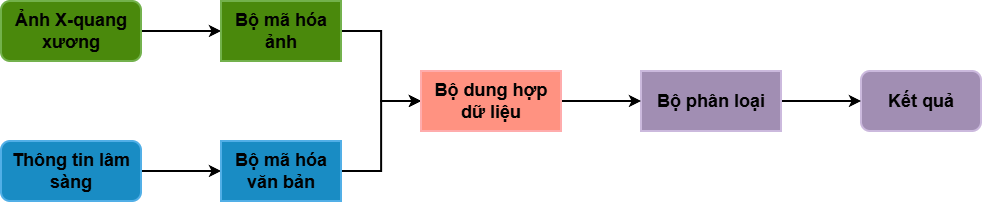
\includegraphics[width=1\linewidth]{images/Pipeline.png}
%     \caption{Khung chương trình tổng quát cho một hệ thống phân loại ảnh sử dụng học sâu đa phương thức}
%     \label{fig:pipeline}
% \end{figure}
% \subsection{Phạm vi nghiên cứu}
% Đề tài tập trung nghiên cứu các bài toán phân loại trên ảnh X-quang kết hợp với thông tin văn bản lâm sàng. Dữ liệu văn bản được sử dụng bao gồm báo cáo đọc ảnh, thông tin lâm sàng và các mô tả liên quan đến bệnh nhân.

% Nghiên cứu chủ yếu sử dụng các bộ dữ liệu cặp ảnh – văn bản đã được công bố công khai cùng với bộ dữ liệu nội bộ được cung cấp thông qua hợp tác với bệnh viện tại Thành phố Hồ Chí Minh. Các bộ dữ liệu này được sử dụng nhằm đánh giá hiệu năng, khả năng tổng quát hóa và tính hiệu quả của mô hình đề xuất thông qua các độ đo phổ biến trong bài toán phân loại.

% Đề tài không tập trung vào các bài toán khác như phát hiện đối tượng, phân đoạn ảnh hay sinh báo cáo y khoa tự động.

\pagebreak

\section{Giới thiệu bài toán}

Bài toán được nghiên cứu trong đề tài là bài toán phân loại đa nhãn ảnh X-quang sử dụng học sâu đa phương thức (multimodal deep learning). Mục tiêu của hệ thống là dự đoán các loại bệnh hoặc tổn thương dựa trên đồng thời dữ liệu hình ảnh X-quang và thông tin văn bản lâm sàng liên quan.

\begin{itemize}
  \item \textbf{Đầu vào (Input):} Hệ thống nhận vào các nguồn dữ liệu sau:

  \begin{itemize}
    \item Ảnh X-quang của bệnh nhân:
    \[
        x^{img} \in \mathrm{R}^{H \times W \times C}
    \]
    trong đó:
    \begin{itemize}
        \item $H, W$: chiều cao và chiều rộng ảnh,
        \item $C$: số kênh màu của ảnh.
    \end{itemize}

    \item Thông tin văn bản lâm sàng gồm các báo cáo đọc ảnh của bác sĩ đọc ảnh, lời khai bệnh nhân và lịch sử bệnh lý được biểu diễn dưới dạng chuỗi token:
    \[
        x^{txt} = \{w_1, w_2, ..., w_T\}
    \]
    trong đó:
    \begin{itemize}
        \item $w_t$: token thứ $t$,
        \item $T$: số lượng token trong văn bản.
    \end{itemize}

    \item Tập nhãn được định nghĩa trước:
    \[
        \mathcal{Y} = \{y_1, y_2, ..., y_K\}
    \]
    với $K$ là số lớp bệnh cần phân loại.
  \end{itemize}

  \pagebreak

  \item \textbf{Đầu ra (Output):} Hệ thống sinh ra:

  \begin{itemize}
    \item Các nhãn dự đoán cuối cùng, được sắp xếp theo thứ tự:
    \[
        y^{*} = \arg\max_{k \in \{1,...,K\}} \hat{y}_k
    \]

    \item Bản đồ nhiệt trực quan hóa trên ảnh nhằm giải thích dự đoán của mô hình
  \end{itemize}
\end{itemize}

\section{Sơ đồ chung của hệ thống}
Hệ thống học sâu đa phương thức được đề xuất bao gồm bốn thành phần chính: bộ mã hóa ảnh, bộ mã hóa văn bản, bộ dung hợp dữ liệu và bộ phân loại. Sơ đồ tổng quan của hệ thống được thể hiện ở Hình \ref{fig:pipeline}.
\begin{figure}[H]
    \centering
    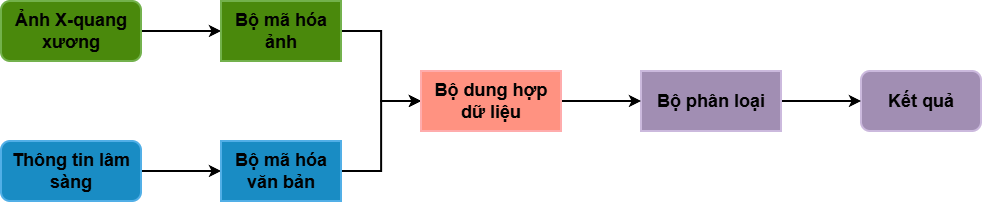
\includegraphics[width=1\linewidth]{images/Pipeline.png}
    \caption{Khung chương trình tổng quát cho một hệ thống phân loại ảnh sử dụng học sâu đa phương thức}
    \label{fig:pipeline}
\end{figure}


% \subsection{Ý nghĩa và tính cần thiết của bài toán}
% Trong thực tế lâm sàng, việc chẩn đoán bệnh không chỉ phụ thuộc vào thông tin hình ảnh mà còn yêu cầu kết hợp với các dữ liệu lâm sàng khác nhằm đưa ra đánh giá toàn diện về tình trạng bệnh nhân. Việc nghiên cứu các mô hình đa phương thức có khả năng khai thác đồng thời dữ liệu hình ảnh và văn bản có ý nghĩa quan trọng trong việc hỗ trợ bác sĩ nâng cao độ chính xác chẩn đoán, giảm thời gian phân tích và tăng khả năng phát hiện bệnh ở giai đoạn sớm.

% Ngoài ra, các hệ thống hỗ trợ chẩn đoán có khả năng giải thích còn giúp tăng tính minh bạch trong quá trình suy luận của mô hình, từ đó tạo điều kiện thuận lợi cho việc ứng dụng trong môi trường y tế thực tế.

% \subsection{Các thách thức trong bài toán}

% Mặc dù các mô hình học sâu đa phương thức đã đạt được nhiều kết quả tích cực, bài toán vẫn tồn tại nhiều thách thức cần được giải quyết:

% \begin{itemize}
%   \item Sự khác biệt về đặc trưng giữa dữ liệu hình ảnh và dữ liệu văn bản gây khó khăn cho quá trình học biểu diễn chung, yêu cầu một cơ chế dung hợp hiệu quả.
%   \item Dữ liệu y tế thường có số lượng hạn chế và mất cân bằng giữa các lớp bệnh, đặt ra yêu cầu đặc biệt về thiết kế mô hình để tận dụng tối đa thông tin có sẵn.
%   \item Trong thực tế lâm sàng, luôn có tỉ lệ xuất hiện những loại bệnh mới nằm ngoài dữ liệu huấn luyện, đặt ra yêu cầu về khả năng tổng quát hóa và thích ứng của mô hình.
%   \item Khả năng giải thích của mô hình vẫn còn hạn chế, gây khó khăn cho việc triển khai trong thực tế lâm sàng.
% \end{itemize}

% \subsection{Các hướng tiếp cận hiện có}
% Các nghiên cứu hiện nay chủ yếu tiếp cận bài toán theo ba hướng chính:

% \begin{itemize}
%     \item Các phương pháp đa phương thức kết hợp dữ liệu hình ảnh và văn bản thông qua các chiến lược dung hợp đặc trưng nhằm khai thác mối tương quan giữa các phương thức dữ liệu.
%     \item Các mô hình ngôn ngữ thị giác quy mô lớn được huấn luyện trước trên dữ liệu đa phương thức nhằm học biểu diễn chung giữa ảnh và văn bản.
%     \item Các mô hình ngôn ngữ lớn đa phương thức được huấn luyện trên nhiều tác vụ khác nhau nhằm tăng khả năng suy luận, hiểu ngữ cảnh và hỗ trợ ra quyết định trong các bài toán y tế phức tạp.
% \end{itemize}

% Mặc dù đã đạt được nhiều kết quả khả quan, các nghiên cứu hiện nay phần lớn chỉ tập trung giải quyết riêng lẻ từng bài toán như học với ít mẫu (few-shot learning) hoặc phát hiện dữ liệu ngoài phân phối (out-of-distribution detection), trong khi vẫn còn thiếu các phương pháp có khả năng xử lý đồng thời các thách thức này trong một khuôn khổ thống nhất. Bên cạnh đó, nhiều phương pháp hiện tại vẫn chưa khai thác hiệu quả mối tương quan ngữ nghĩa giữa dữ liệu hình ảnh và văn bản, đồng thời còn hạn chế về khả năng giải thích quá trình suy luận và đưa ra quyết định của mô hình.
% \section{Các câu hỏi nghiên cứu}

% \section{Đóng góp của luận văn}

% \section{Bố cục luận văn}
% Khóa luận được trình bày một cách hệ thống và logic qua 5 chương, dẫn dắt người đọc từ tổng quan lý thuyết đến thực nghiệm chi tiết và kết luận:

% Chương 1: Giới thiệu. Chương này cung cấp cái nhìn tổng quan về bối cảnh nghiên cứu, xác định rõ vấn đề cần giải quyết, mục tiêu, phương pháp tiếp cận và những đóng góp chính của đề tài. Đây là phần nền tảng định hướng cho toàn bộ nội dung khóa luận.

% Chương 2: Các công trình nghiên cứu liên quan. Chương này đi sâu vào nền tảng kiến thức và các công trình đi trước. Nội dung bao gồm các kiến thức nền tảng về Học sâu (Deep Learning), Mạng nơ-ron tích chập (CNNs), và đặc biệt là cơ chế Attention và Transformer. Trọng tâm của chương là lý thuyết về Học đa phương thức (Multimodal Learning), kiến trúc của các mô hình ngôn ngữ trực quan và các kỹ thuật kết hợp dữ liệu được áp dụng.

% Chương 3: Phương pháp đề xuất. Đây là chương trọng tâm mô tả chi tiết quy trình xây dựng hệ thống. Tại đây, nhóm sẽ trình bày cụ thể về kiến trúc mô hình Med-VLM được lựa chọn, quy trình xử lý dữ liệu đầu vào (cả ảnh và văn bản), thiết kế các hàm mất mát (loss functions), và chiến lược huấn luyện mô hình (training strategy). Các sơ đồ khối và thuật toán sẽ được mô tả chi tiết để minh họa cho giải pháp.

% Chương 4: Thực nghiệm và Kết quả. Chương này trình bày về bộ dữ liệu được sử dụng, thiết lập môi trường thực nghiệm và các chỉ số đánh giá (metrics) như Accuracy, F1-Score, AUC-ROC. Kết quả thực nghiệm sẽ được phân tích sâu, so sánh đối chiếu với các phương pháp khác để làm rõ ưu nhược điểm của mô hình đề xuất. Các phân tích sai số (error analysis) cũng được thực hiện để hiểu rõ hành vi của mô hình.

% Chương 5: Kết luận và Hướng phát triển. Chương cuối cùng tổng kết lại những kết quả đạt được so với mục tiêu ban đầu, nhìn nhận thẳng thắn những hạn chế còn tồn tại của hệ thống và đề xuất các hướng nghiên cứu tiếp theo để hoàn thiện và mở rộng ứng dụng trong tương lai.